In this section, the processing layer's hardware and software design are delineated. The layer comprises a PLC, Ethernet switch, and a Robot Controller interconnected to facilitate communication and decision-making processes. The processing layer comprises of connection and communication between the PLC and the robot controller primarily. In order to program the PLC to do the required tasks, GX Works3 (software) and RTToolbox (software) are jointly used. A program written in ladder logic controls the logic for the air compressor and light tower. The program inside the PLC is written from the PC and executed. The instructions are passed onto the controller and directs the robot to move its joints according to the program. 


\subsection{Layer Hardware}
The hardware involved with the processing layer include a MELSEC Programmable Logic Controller, issued by Mitsubishi. The PLC is a specialized computer used in industrial automation and is paired with software to make decisions based on the instruction from the Host PC, signals from the switches. Finally, the PLC is equipped with an ethernet socket that enables communication between the Host PC and PLC through an Ethernet switch. The robot controller controls the actions and behaviors of robotic systems through joints movement, transforming programmed instructions into precise and efficient movements to fulfill a wide range of industrial tasks and applications. 

\subsection{Layer Operating System}
The operating systems required by the layer are dependent on the specific components. The host PC runs on Windows 10 and PLC is on Real Time Operating System (RTOS).

\subsection{Layer Software Dependencies}
The Host PC uses RT ToolBox for ladder logic, GX Works3 to controlled movement of joints, and it uses Windows 10 as operating system. 

\subsection{PLC}
PLCs provide a centralized platform for controlling and programming the movements of the RV-8 robot. They execute logic sequences that regulate the robot's motions, trajectories, and speeds, ensuring precise and coordinated operation in the manufacturing environment. PLCs interface with sensor systems to enable adaptive control schemes and provide input to RV-8 robots. They have safety features such emergency stop connections to validate the work cell's safety state and light towers to show the operating condition. 

\begin{figure}[h!]
	\centering
 	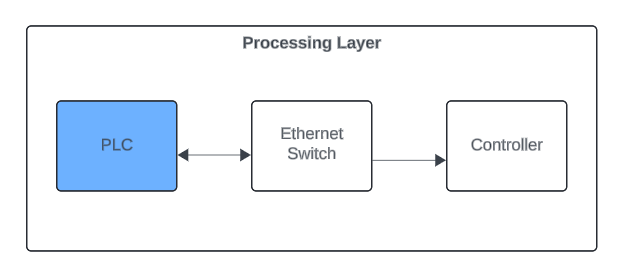
\includegraphics[width=0.6\textwidth]{images/PLC_Processing.png}
 \caption{ PLC Subsystem}
\end{figure}

\subsubsection{Subsystem Hardware}
The Mitsubishi Electric MELSEC iQ-F FX5UC-32MT/DSS-TS PLC is a compact unit featuring 32 I/O points, 16 digital inputs, and 16 digital outputs, all operating at 24Vdc and Ethernet communication capabilities. The PLC also has an external relay switch FX5-8EYR/ES with 8 digital outputs.


\subsubsection{Subsystem Operating System}
Operating on a real-time operating system (RTOS), the PLC ensures precise timing and reliable execution of control logic.

\subsubsection{Subsystem Software Dependencies}
Software tools such as GX Works and MRConfigurator2, provided by Mitsubishi Electric, enable the programming and configuration of the PLC for control tasks.

\subsubsection{Subsystem Data Processing}
The PLC processes sensor feedback and command signals in real-time, executing control logic to coordinate the movements of the robotic arm and additional axis. Communication with the host PC via TCP/IP facilitates efficient data exchange for seamless system operation.


\subsection{Ethernet Switch}
Ethernet Switch plays an important role in facilitating communication and data exchange within the control system. In order to provide compatibility with a variety of devices and controllers and to enable smooth integration with current automation systems, the switch supports a wide range of communication protocols, including TCP/IP. 
\begin{figure}[h!]
	\centering
 	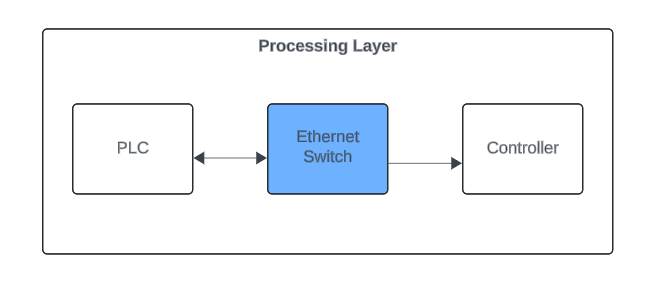
\includegraphics[width=0.65\textwidth]{images/Ethernet_Processing.png}
 \caption{Ethernet Switch Subsystem}
\end{figure}

\subsubsection{Subsystem Hardware}
The subsystem uses Ethernet switch board with 8 sockets.

\subsubsection{Subsystem Software Dependencies}
Uses Windows for it's user-interface.


\subsection{Robot Controller}
The movements, actions, and functions of one or more robotic arms or manipulators are coordinated and controlled by a robot controller, which acts as the control system of a robotic system. Controlling the robotic arm's motion is the main responsibility of the robot controller. The robot's joints are controlled by motors and actuators that it creates commands to drive, allowing for precise and coordinated movement in three dimensions. It support TCP/IP communication protocol for interfacing with other devices and robot arm to communicate. It is connect with PLC via Ethernet switch, which acts as slave device and PLC as master device, as PLC processes the data from the slave device to performs control actions using robot controller.  
The back panel of the robot controller has 2 connectors (CNUSR11 and CNUSR12) pins that allow for other connections, such as emergency stop (e-stop) capabilities, which guarantees rapid stops to the robot arm's movements in an emergency. It also makes it easier to attach a light tower, which provides a visible signal of the operational state of the working cell. The robotic system's overall safety and efficiency are improved by this combination of safety features, which offer real-time monitoring and quick response times to guarantee a safe working environment.

\begin{figure}[h!]
	\centering
 	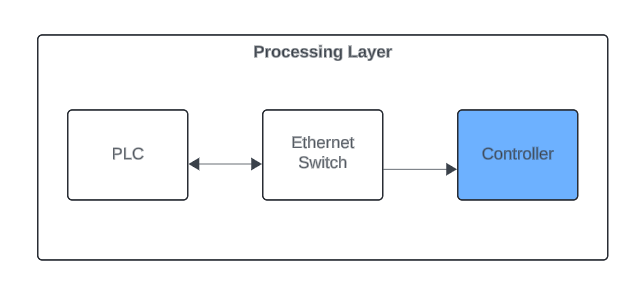
\includegraphics[width=0.65\textwidth]{images/Controller_Processing.png}
 \caption{Robot Controller Subsystem}
\end{figure}

\subsubsection{Subsystem Hardware}
It contains network card for CC-Link.

\subsubsection{Subsystem Operating System}
Operates on Host PC, which uses Windows as it's operating system. 

\subsubsection{Subsystem Software Dependencies}
It uses RT-ToolBox for it's programming, also called Ladder logic programming. 

\subsubsection{Subsystem Programming Languages}
Programming languages supported by GXWorks, including ladder logic, function block diagrams, and structured text, are utilized for developing control algorithms tailored to the application. RT ToolBox is written in MELFA BASIC VI.


\subsubsection{Subsystem Data Processing}
No data processing is done by Robot controller, it uses operates on PLC logical output. 